\section{Del 1}

Vi har fundet et lydklip af vindmølle støj med en sampling frekvens på 48kHz og et lydklip af en PC blæser med en sampling frekvens på 44.1kHz. Udvalgte 10 sekunder af disse filer er plottet i \autoref{fig:wm_10s} og \autoref{fig:pc_10s}.

Det kan ses at vindmøllen svinger i lydstyrke ca.\ en gang hvert 1.5 sekund, mens blæseren kører med en mere konstant (og lavere) lydstyrke.

\begin{figure}[h]
\centering
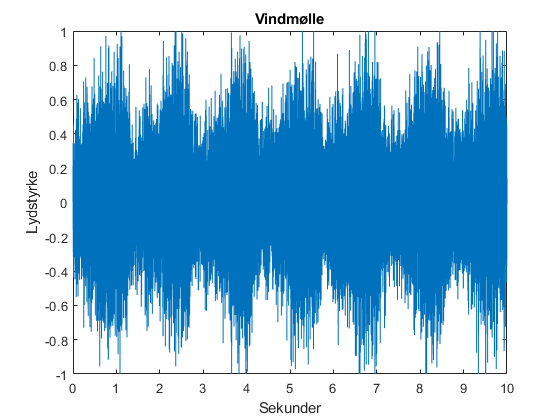
\includegraphics[width=\textwidth]{figures/Windmill_10s}
\caption{10s lyd fra vindmølle}%
\label{fig:wm_10s}
\end{figure}

Ud fra sampling frekvenserne kan man beregne frekvensopløsningen med 
\begin{equation}
\Delta f = \frac{f_{sample}}{N}
\end{equation}
hvor N er antal samples, og derfor også antallet af frekvens bins.
Da begge lydklip er 10 sekunder består de af $f_{sample}*10$ samlpes, hvorfor samplefrekvensen bliver: 
\begin{equation}
\Delta f = \frac{f_{sample}}{f_{sample}*10} = 0.1 Hz
\end{equation}
For vindmøllen, med $f_{sample}=48000$ og $N=480000$ : $\Delta f_{wm} = \frac{48000}{480000} = 0.1$Hz.

\begin{figure}[h]
\centering
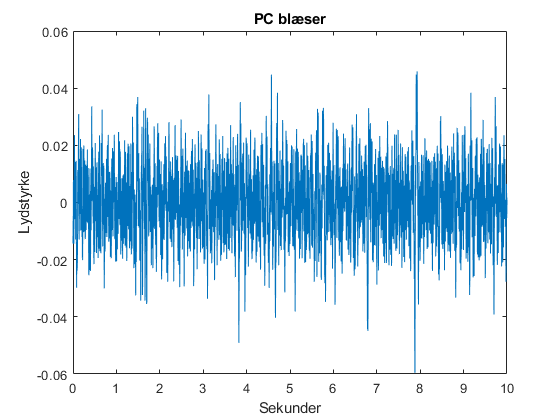
\includegraphics[width=\textwidth]{figures/pcFan_10s}
\caption{10s lyd fra PC blæser}%
\label{fig:pc_10s}
\end{figure}

\newpage

\section{Del 2}

\autoref{fig:WM_freq} og \autoref{fig:pc_freq} viser frekvensspektret for de to lydklip. Det ses at begge spektre har samme bue form, dog med forskellige toppunkter (vindmøllen topper ved ca. 200 Hz, mens blæseren topper ved 10Hz), og at vindmøllens spektrum topper ved en højere frekvens end PC blæserens spektrum. Der er også adskillige peaks i de to spektre. Vindmøllen har to kraftige bredde peaks ved ca. 10 og 100 Hz, samt flere mindre og smallere peaks, mens blæseren har en enkelt kraftig, men tynd peak ved ca 40Hz. 

\begin{figure}[h]
\centering
\includegraphics[width=0.8\textwidth]{"figures/Windmill_frekvens"}
\caption{Frekvens spektrum af vindmølle}
\label{fig:WM_freq}
\end{figure}

\begin{figure}[h]
\centering
\includegraphics[width=0.8\textwidth]{"figures/pcFan_frekvens"}
\caption{Frekvens spektrum af PC blæser}
\label{fig:pc_freq}
\end{figure}


\section{Del 3}

Til at udregne lavfrekvens- og højfrekvens-energi bruges ligningerne:

\begin{equation}
E_{low} = \frac{2}{N} \sum_{f=0}^{80Hz} |X(f)|^2
\end{equation}

\begin{equation}
E_{high} = \frac{2}{N} \sum_{f=80Hz}^{max} |X(f)|^2
\end{equation}

For vindmøllen giver det: $E_{low} = 129.6$ og  $E_{high} = 66934$, mens de for blæseren giver  $E_{low} = 59.04$ og  $E_{high} = 65.81$.\\

For vindmøllen fås $\frac{E_{low}}{E_{high}} = 0.0019$ og fov PC blæseren $\frac{E_{low}}{E_{high}} =0.8972$.\\

I begge tilfælde ses det at der er mere energi i de høje frekvenser, end i de lave, og at der for vindmøllen er meget mere energi ved høje frekvenser. Dette ses ved at frekvens spektret topper over 80Hz, mens PC blæseren har energien mere ligeligt fordelt.


\section{Del 4}

Hvis signalet forkortes vil de laveste frekvenser ikke kunne medregnes, da de ville blive mindre end frekvens opløsningen. Dette forventes at forskyde energis-forholdet mod mere højfrekvent energi. Tilsvarende kan en forlængelse af signalet  forventes at ændre forholdet til fordel for den lavfrekvente energi, da lavere frekvense nu kan medregnes. Det er dog usandsynligt at en ændring vil kunne måles, da energien i de lave frekvenser er lille.\\

For vindmøllen viser det målte energi forhold at det meste energi er i frekvenser over 80Hz, så med mindre der er en enorm mængde energi med frekvenser under 0.1 Hz vil det ikke forventes en betydelig ændring.
